\documentclass{llncs}

\usepackage{url}
\usepackage[pdftex]{graphicx}
\usepackage{listings}
\usepackage{verbatim}
\usepackage[lined,linesnumbered,algochapter]{algorithm2e}
\usepackage{tikz}
\usetikzlibrary{arrows,automata}
\usepackage{xspace}
\usepackage {pdfsync}
\usepackage{amsmath}
\usepackage{tabularx}

\usepackage{ngerman}
\usepackage[ngerman, english]{babel}
\usepackage{bibgerm,cite}       % Deutsche Bezeichnungen, Automatisches Zusammenfassen von Literaturstellen
\usepackage[ngerman]{varioref}  % Querverweise

\usepackage{ammalang}

\setcounter{secnumdepth}{2}
\setcounter{tocdepth}{3}

% define custom macros for specific formats or names
\newcommand{\uml}[1]{\texttt{#1}}
\newcommand{\cd}{\textsf{Class Diagram}}

\begin{document}
\pagestyle{plain}
\pagenumbering{roman}

\title{Towards Systematic Mutations for and with ATL Model Transformations\footnote{This work has been created in the context of the course ``188.952 Advanced Model Engineering (VU 2,0)'' in SS15.}}


%&&&&&&&&&&&&&&&&&&&&&&&&&&&&&&&&&&&&&&&&&&&&&&&&&&&&&&&&&&&&&&&&&&&&&&&&
% Name and address of the author
%&&&&&&&&&&&&&&&&&&&&&&&&&&&&&&&&&&&&&&&&&&&&&&&&&&&&&&&&&&&&&&&&&&&&&&&&
\author{Patrick Sommer\inst{1} and Carola Gabriel\inst{2} and Martin Keiblinger\inst{3}}

\institute{Mautner Markhof-Gasse 58/4/31, 1110 Wien \\ \email{e0925011@student.tuwien.ac.at} \\ MatrNr.: 0925011
\and
Leberweg 14/3/16, 1110 Wien \\ \email{e0825992@student.tuwien.ac.at} \\ MatrNr.: 0825992
\and
Mustergasse 54/4/3, 1030 Wien \\ \email{matthias@tuwien.ac.at} \\ MatrNr.: 0426553
}

\maketitle

\begin{abstract}

Faults in model transformations will produce faults in models. The correction of
the defective models is often very expensive. This result affects the quality
of the end product. This is why model transformations has to be correctly tested
to maintain product quality. For this mutation testing is a popular technique.  The mutation testing of model transformations have to be developed and for this a suite of mutation operators for the Atlas Transformation language (ATL) is needed. In this paper a set of mutation operators are implemented and the solutions of the implementations are discussed and evaluated regarding effectiveness.

\end{abstract}

%&&&&&&&&&&&&&&&&&&&&&&&&&&&&&&&&&&&&&&&&&&&&&&&&&&&&&&&&&&&&&&&&&&&&&&&&
% Table of contents
% Activate or deactivate this according to the guideline instructor
%&&&&&&&&&&&&&&&&&&&&&&&&&&&&&&&&&&&&&&&&&&&&&&&&&&&&&&&&&&&&&&&&&&&&&&&&
\tableofcontents
%\thispagestyle{plain}
\newpage

\pagenumbering{arabic}

\section{Introduction}

Model transformation allows to synthesize software artifacts from model definitions and ease other software engineering tasks by automating them.

This abstraction eases incremental processes like:\cite{Sendall:2003}
\begin{itemize}
	\item Reverse engineering models e.g. in the process of replacing a legacy system. The resulting artifact can be tested and if results of the legacy and the new system are found only the model has to be changed.
	\item Refactoring models
	\item et cetera
\end{itemize}

Therefore the quality of the overall software solution is determined by the quality of the models and the resulting model transformations.\cite{Hutchinson:2011} As a consequence testing the transformations for correctness is an essential part to achieve the best possible quality of the software.\cite{troya:2015}

To check the quality of a software it has to be tested. Software testing is a process, or a series of engineered processes  to check if a program does what it is designed for and that it does not do anything unintended.\cite{Myers:2004} Model based testing (MBT) is a variant of this software testing process. Test cases are not written by the programmer directly. The programmer only creates a model of the requirements and in a second step the test cases are generated based on this model.\cite{Utting:2012}

Mutation testing or mutation analysis is a fault-based testing technique. It
applies changes to the input model and creates a mutant. Every mutant represents a faulty
program. In the best case these changes, which are applied by the mutator, represent mistakes a programmer would make. It has been proven that mutation testing is useful as testing approach but also as:\cite{mutationssurvey:yue}

\begin{enumerate}
	\item Generate input models as test data.
	\item Generate mutants of model transformations.
\end{enumerate}

\subsection{Problem}

To make mutation testing an effective testing method a complete set of mutation operators and a large number of mutated model transformations has to exist. Due to the needed size of these sets it's to expensive to create them manually. Also the execution of the different models against the test data is very time-consuming.

Therefore automation is required for:

\begin{enumerate}
	\item generation of a set of mutation operators.
	\item generation of mutated model transformations.
\end{enumerate}

Furthermore, the computational costs of the executions have to be lowered.

\subsection{Contribution}

Troya et. al. contributed three aspects.

\begin{enumerate}
	\item They have defined a general languagecentric synthesis approach by defining a set of mutation operators based on ATL. 
	\item They made a concept and build a first version of a framework utilizing Higher order transformations for generating mutants.\cite{Paige:2009}
	\item They integrated techniques\cite{Bergmayr:2014} for incremental model transformation execution in their framework.
\end{enumerate}

We contribute further implementations of mutation operators and small tests.

\section{Background}

\subsection{Model transformation in MDE}

This work is focused on mutation testing for model transformations. The basic idea of mutation testing in software engineering is not to test the resulting software itself but the test cases.

Good test cases should be able to identify mutants. In he jargon of mutation testing the mutations are \emph{killed}. Killing means recognizing differing results of the original system under test (SUT) and tested mutants.\cite{MatMottu2006}

The process of mutation testing consists of four components: 
\begin{itemize}
	\item \textit{Test data} as input for the original programm P and its mutants.
	\item The original program \textit{P}
	\item The \textit{mutants} of P.
	\item An \textit{oracle} which is able to decides if results differ and which is therefore able to identify mutants.
\end{itemize}

The goal of the process\ref{fig:Mutation_Process} is to \textit{kill} or identify faulty versions of the original program. If a mutant outputs the same data for the same input data as the original program it's called \textit{equivalent}. In this case this mutant has to be removed from the set of mutants under test.

The last step is to assess how good the tests are and check if they should be improved. Assume \textit{KM} is the set of the killed mutants, \textit{M} is the set of all mutants and \textit{EM} is the set of all identified, equivalent mutants then the mutation score \textit{MS} is calculated like this:\cite{mutationssurvey:yue}

\begin{equation}
	MS = \frac{\left|KM\right|}{\left|M\right| - \left|EM\right|}
	\label{eq:ms}
\end{equation}

If this value is too small the tests have to be improved. 

The success of this method depends on the set of mutants used in the process. Manual creation of mutants is a tedious and time consuming task. Therefore a quick, reliable and efficent creation of mutants is proposed in \cite{troya:2015}.

Troya et al. build upon ATL and higher order transformations (HOT) to create transformations to automatically generate mutants. 

This report shows which additional transformations have been developed and what their goals are. The scope of this work is the mutation generation in the whole process.

\begin{figure}
	\centering
	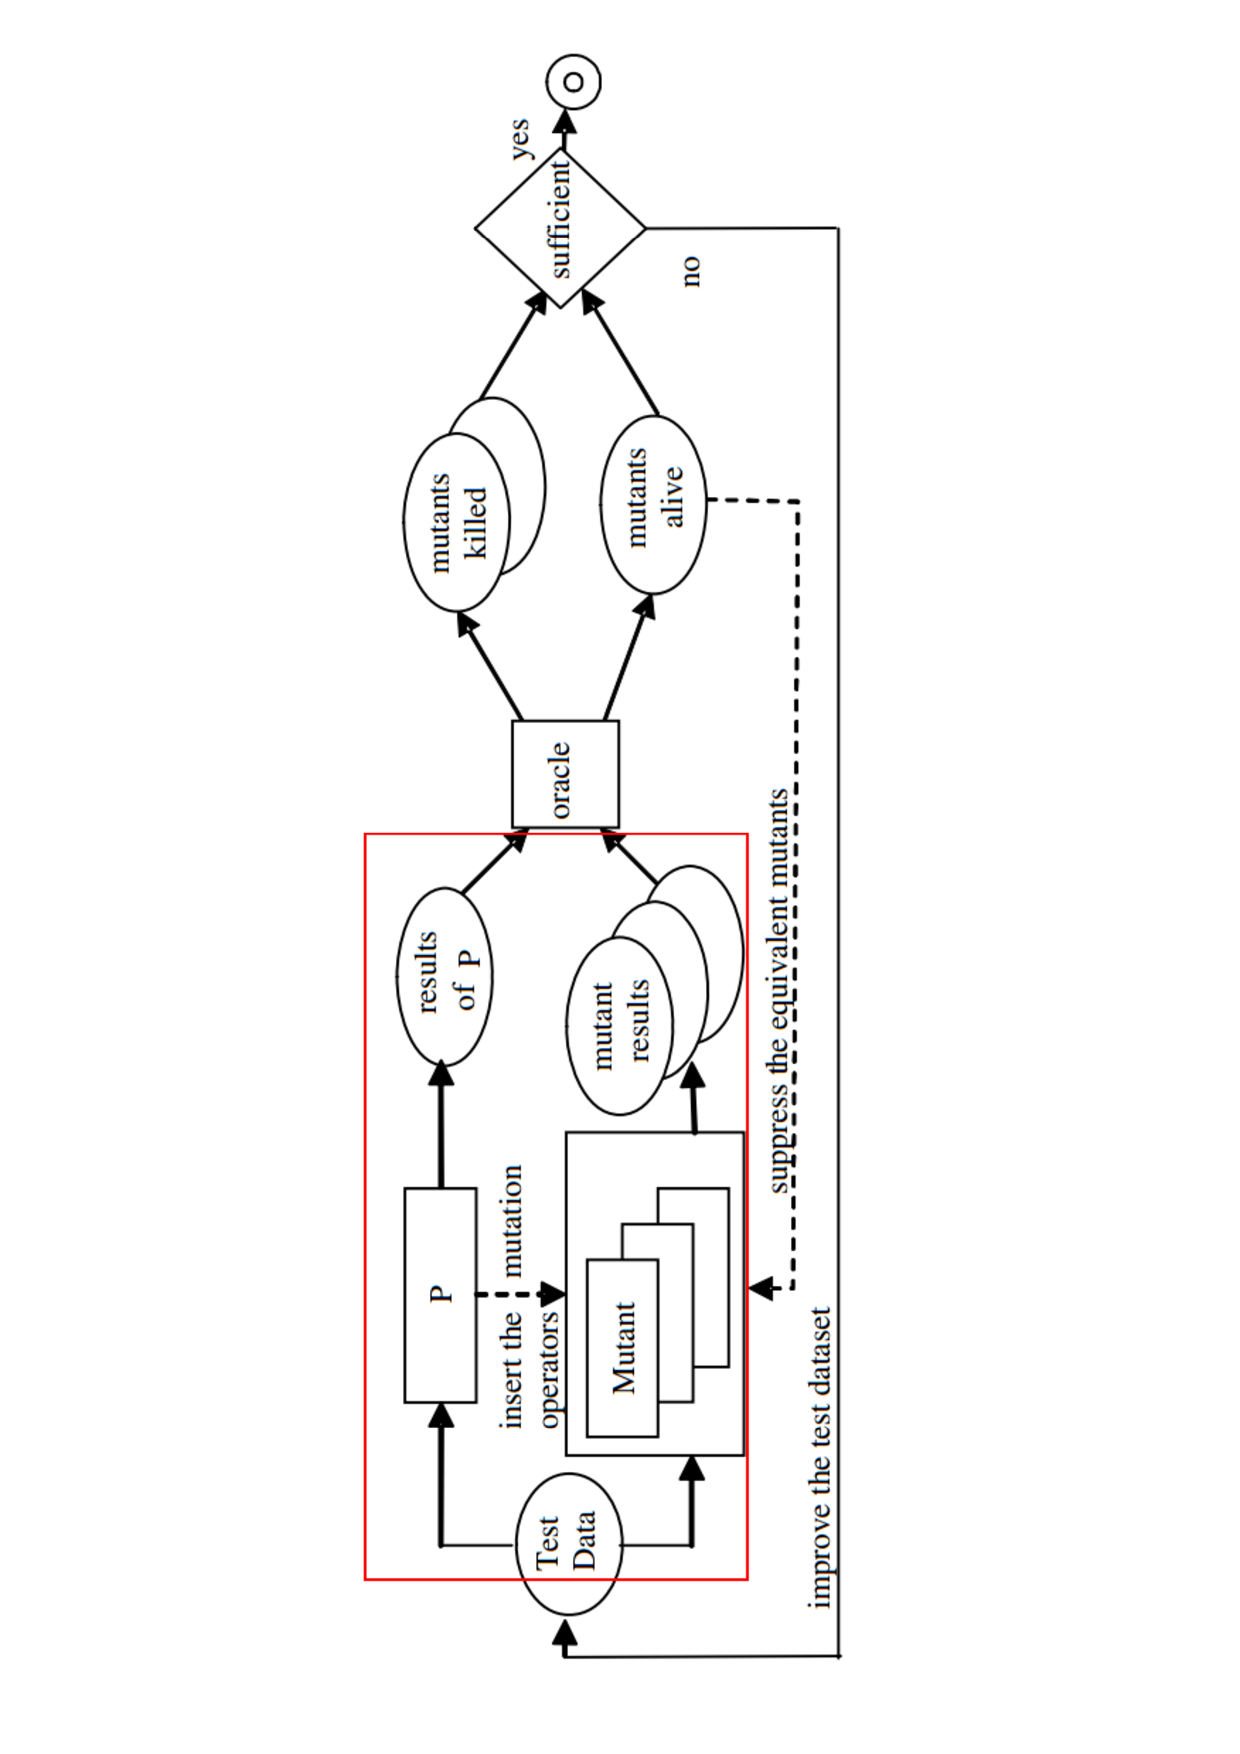
\includegraphics[angle=270,width=1\textwidth]{figures/Marked_Mutation_Process.pdf}
	\caption{The mutation testing workflow contains a feedback loop. The red marked area is the part this paper contributes to.\cite{MatMottu2006}}
	\label{fig:Marked_Mutation_Process}
\end{figure}

Model transformations plays an important role in the Model Driven Engineering
(MDE) approach. Developing model transformation definitions is expected to
become a common task in model driven software development. \cite{atl:frederic}
In this part of the paper we want to explain the basics of the requirements we needed for mutations for and with ATL Model Transformations.

\subsection{Mutation Testing}

Speaking in broader terms, model transformation is the process of synthesizing one or more models from one or more input models. To successfully generate output-models it needs a clear understanding of the syntax and the semantic of these models and the relationship between their different entities. Model driven engineering provides a formal framework to define this prerequirements.\cite{Sendall:2003}

At the highest level two main categories of model transformations exist:\cite{Czarnecki03}

\begin{enumerate}
	\item Model to model transformations
	\item Model to code transformations
\end{enumerate}

Model to code transformations take models as input and generate source code as output. There exists two different approaches to synthesize the generated source code. On the one side there is the visitor based approach, which is driven by a model traverse engine which outputs code artifacts when it visits specific points in the model hierarchy. The other approach is the template based appraoch. Therefore a template consists of constant text and parts which dynamically generates text from the input model. The dynamically part expands iterativly.\cite{Czarnecki03}


For model to model transformations there exist multiple strategies:

\begin{itemize}
	\item The \emph{Direct-manipulation approach} offers an internal model representation and tools to manipulate it.
	\item The \emph{relational approach} uses relations, in the sense of the mathematical concept, and mapping rules. In combination with a declerative logic for defining constraints, this is used to produce executable transformations.
	\item The \emph{graph-transformation-based approach} utilizes graph theory. It models entities as nodes and edges in the graph to define model transformations.
	\item The \emph{structure-driven approach} provides the user with a framework to operate on a hierarchy to copy objects and their attributes.
	\item The  \emph{hybrid approach} is the combination of two or more of the above mentioned concepts.
\end{itemize}

\subsubsection{ATL}

ATL is a model transformation language containing a mixture of declarative and
imperative constructs. ATL is applied in the context of the
transformation pattern shown in figure \ref{fig:overview_atl}. In this pattern a source
model Ma is transformed into a target model Mb according to a transformation definition mma2mmb.atl written in the ATL language. This transformation definition is a model conforming to the ATL metamodel. All metamodels conform to the MOF.

\begin{figure}
	\centering
	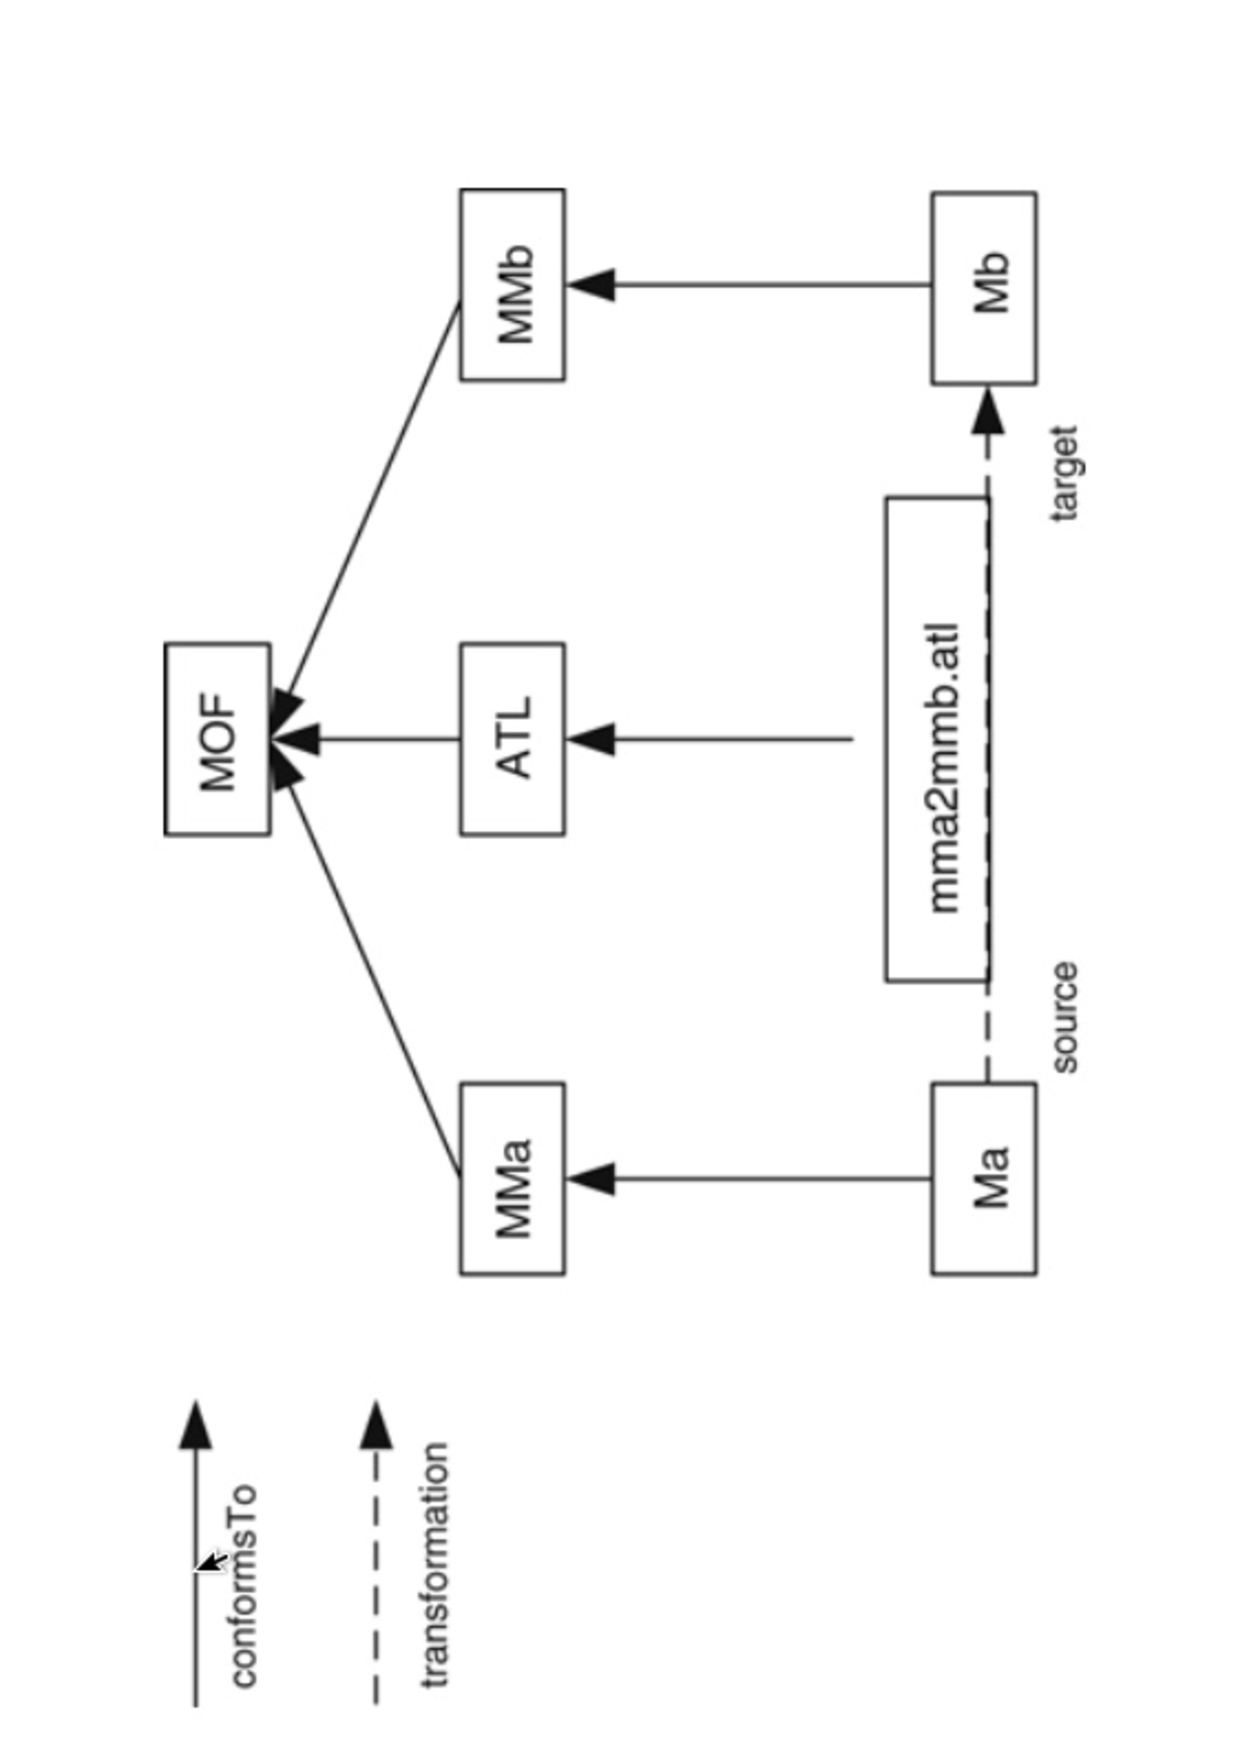
\includegraphics[angle=270, width=1\textwidth,natwidth=610,natheight=642]{figures/Overview_ATL.pdf}
	\caption{Overview of the ATL transformational approach}\cite{atl:frederic}
	\label{fig:overview_atl}
\end{figure}

ATL is a hybrid transformation language. It is encouraged to use a declarative style of specifying transformations. The declarative style of transformation specification has a number of advantages: it is usually based on specifying relations between source and target patterns and thus tends to be closer to the way the developers intuitively perceive a transformation. This style stresses on encoding these relations and hides the details related to selection of source elements, rule triggering and ordering, dealing with traceability, etc. Therefore, it can hide complex transformation algorithms behind a simple syntax.\cite{atl:frederic}

\begin{figure}
	\centering
	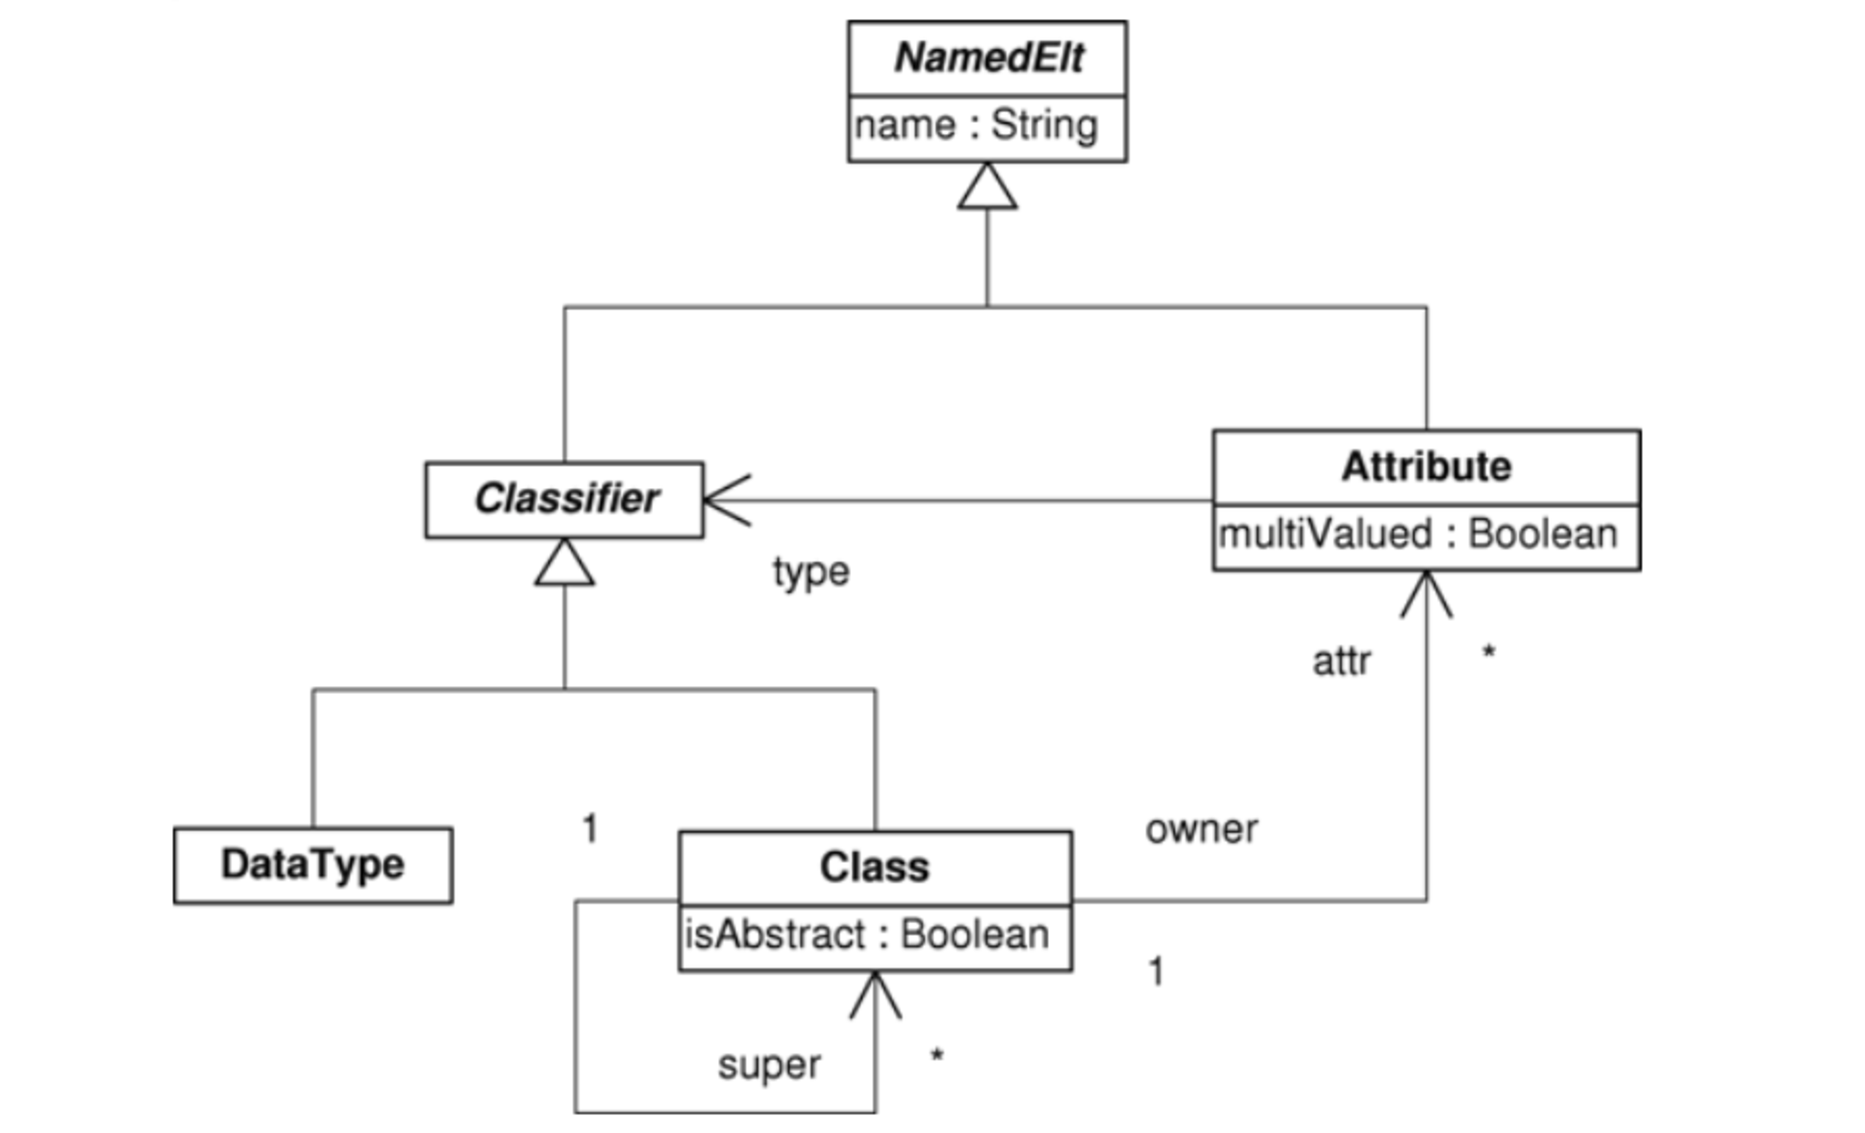
\includegraphics[width=1\textwidth,natwidth=610,natheight=642]{figures/Class_metamodel.pdf}
	\caption{Class metamodel}\cite{atl:frederic}
	\label{fig:class_metamodel_atl}
\end{figure}

The class metamodel is used by ATL transformations \ref{lst:shortexample}
shown in figure \ref{fig:relational_metamodel_atl}\cite{atl:frederic}

\begin{figure}
	\centering
	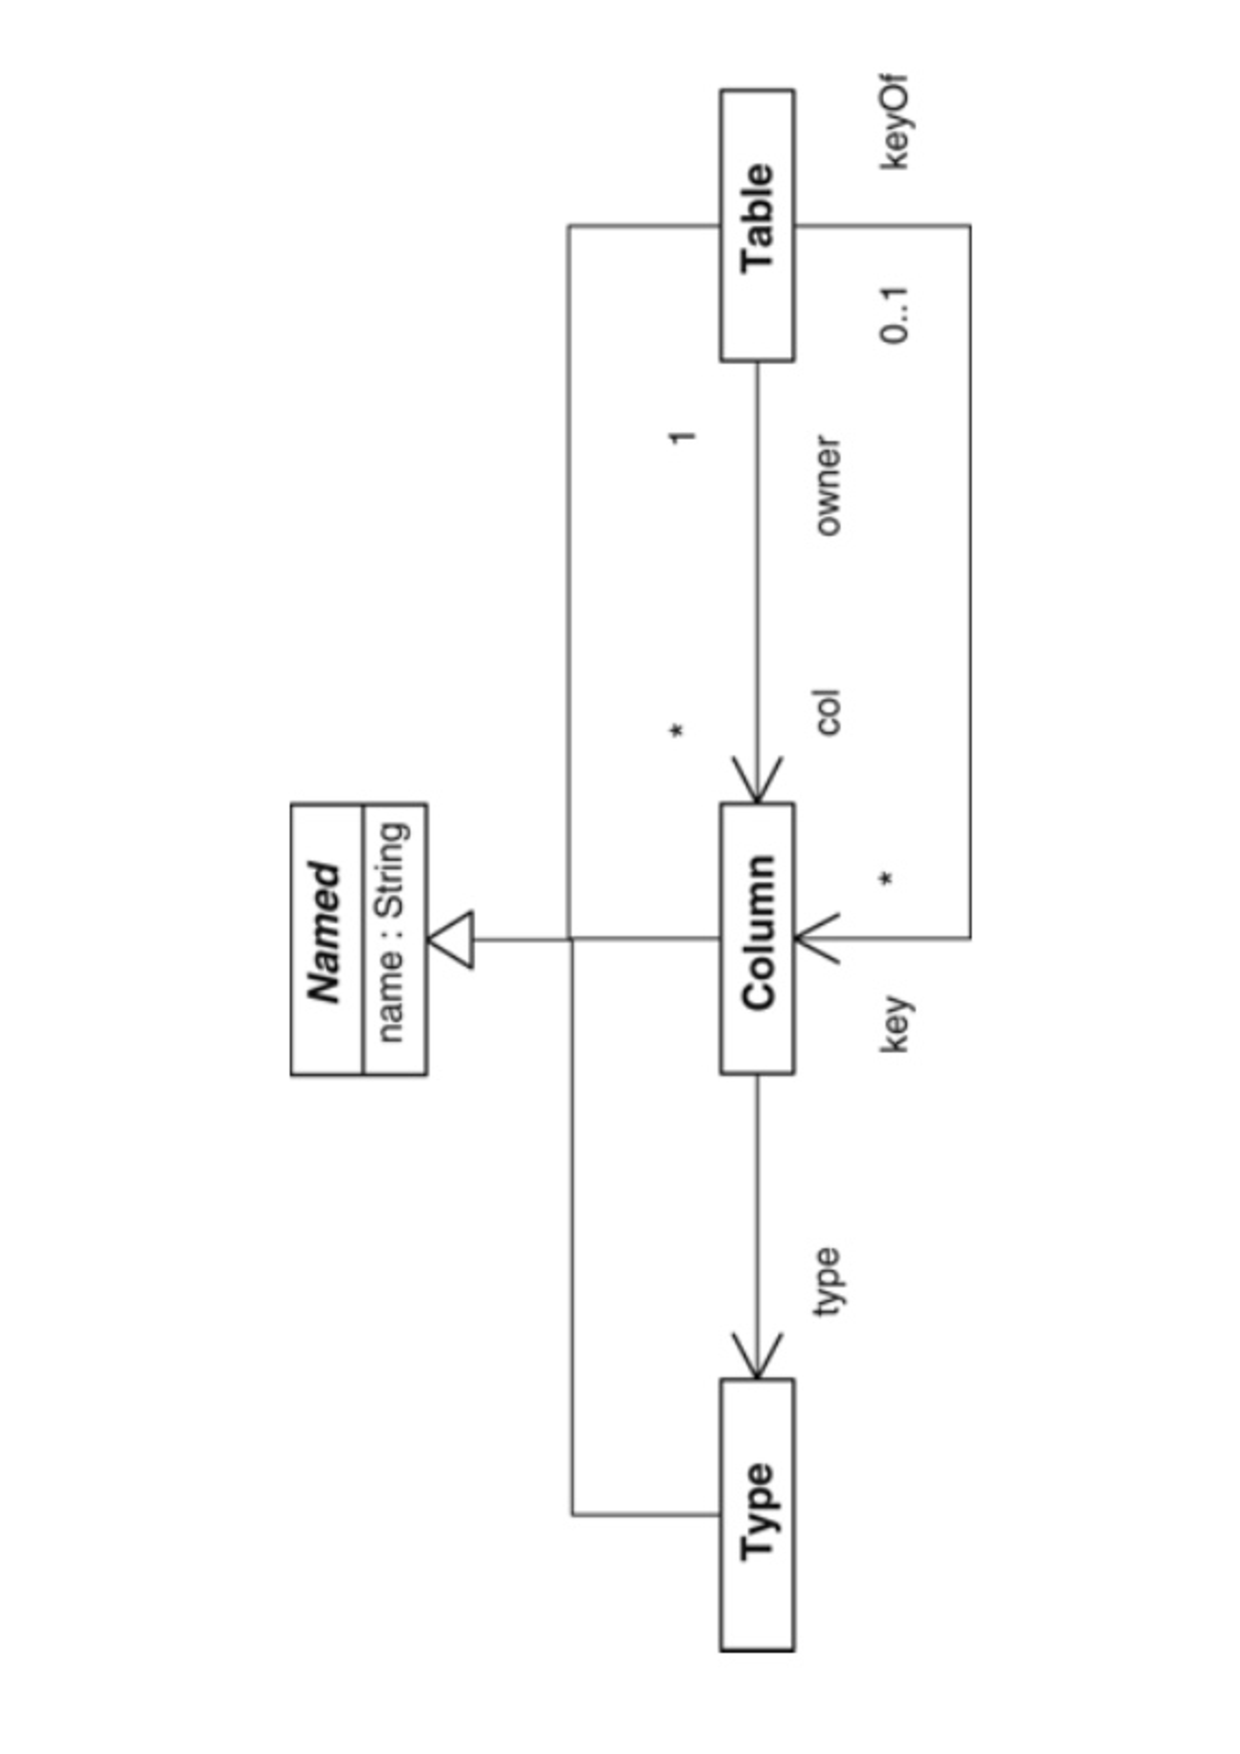
\includegraphics[angle=270,width=1\textwidth,natwidth=610,natheight=642]{figures/Relational_metamodel.pdf}
	\caption{Relational metamodel}\cite{atl:frederic}
	\label{fig:relational_metamodel_atl}
\end{figure}

In this part we want to create a transformation program for a general example
that transforms simple class models to relational models. The source and the
target model are presented in figure \ref{fig:class_metamodel_atl} and figure 
\ref{fig:relational_metamodel_atl}.

\begin{lstlisting}[language=ATL, numbers=left,xleftmargin=5.0ex, caption=Simple example for a ATL transformation, label=lst:shortexample]
//Start Program
module Class2Relational;
create OUT : Relational from IN : Class;

rule Class2Table {
	from
		c : Class!Class
	to 
		out : Relational!Table (
			name <- c.name
		)
}
//End Program
\end{lstlisting}

The source model is the 'IN' model and the target model is 'OUT'. The rule maps the element EntityModel to FormModel.

\subsubsection{Higher Order Transformations}

Higher order transformations are defined as model transformations where the input and/or the output models are transformation models themselves.\cite{Tisi:2009}

Figure \ref{fig:samplefigure_pdf} shows a sample schema of a higher order transformation for transformation modification
in ATL where you can see a good overview for the model transformation with transformation models as input and output models.

 \begin{figure}
	\centering
	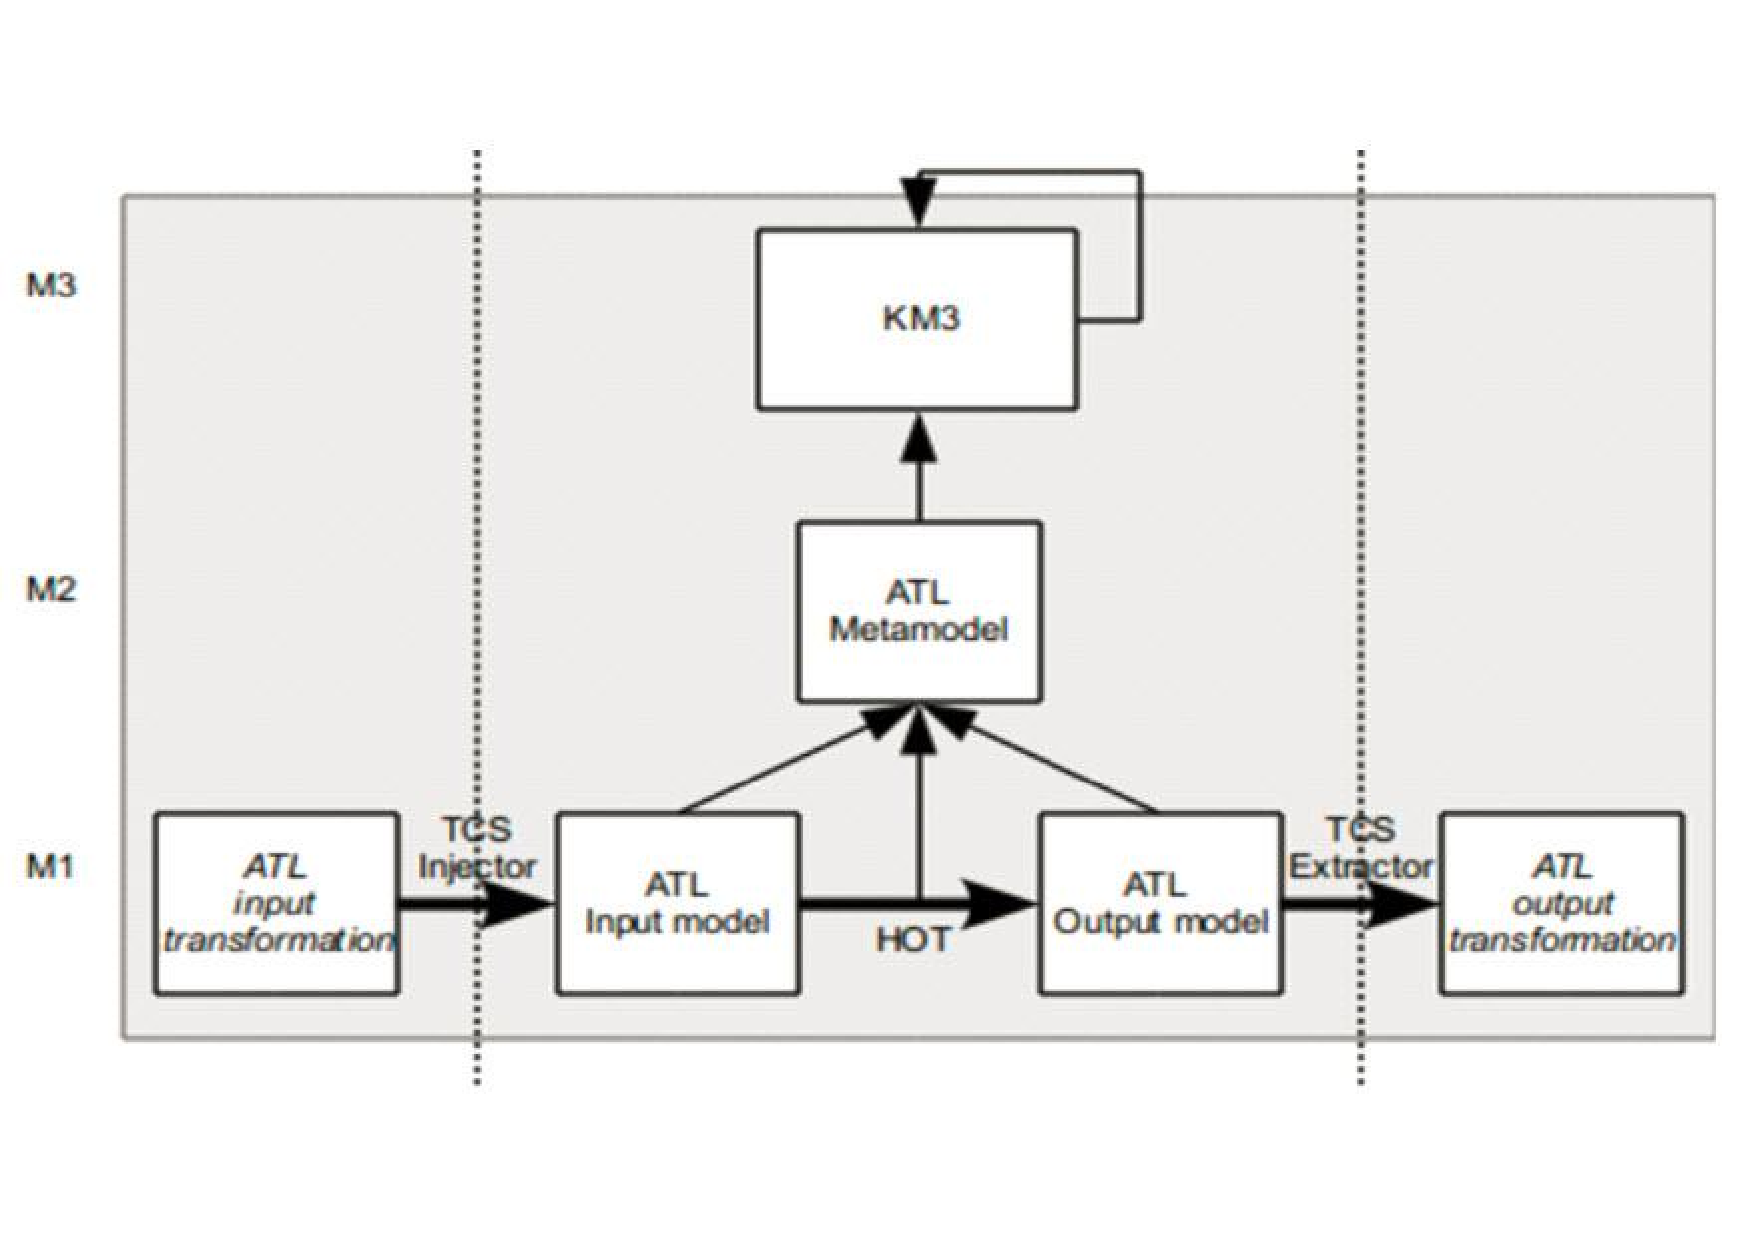
\includegraphics[width=1\textwidth,natwidth=610,natheight=642]{figures/HOT.pdf}
	\caption{Sample schema of a Higher Order Transformations for transformation modification in
	ATL}\cite{misc:ModelingLanguages}
	\label{fig:samplefigure_pdf}
\end{figure}~\cite{misc:ModelingLanguages}

Therefore a transformation model can be:

\begin{itemize}
	\item The input model of a higher order transformation
	\item The output model of a higher order transformation
	\item Both, the input and the output model
\end{itemize}

Tisi et. al \cite{Tisi:2009} identified four transformation patterns for Higher
order transformations:

\begin{itemize}
	\item \textbf{Transformation Synthesis} These Higher order transformations
	generate transformations. If any input is used it is not a transformation.
	\item \textbf{Transformation Analysis} takes transformations as input and generates data of different types as output. The output is never a transformation.
	\item \textbf{Transformation (De)composition} is the integration of multiple transformations of the input and/or integration of transformations as output.
	\item \textbf{Transformation Modification} is defined by modifing an input transformation and generating an output transformation.
\end{itemize}

The focus of this work is on \textit{Transformation Modifications} (short TM). 

Another possibility of a Higher order transformation is a second Higher order
transformation. That means that a Higher order transformation will also be the
input/output of another transformation.

\subsection{Mutations in Model Transformations}
In order to identify the possibilities of mutations in languages we need to know
about the concepts of the languages which can be mutated. This mutation possibilities
are presented in the referenced paper \cite{troya:2015}. For a better overview
 the following table shows the possible mutations for ATL
transformations.\label{fig:mutations_ATL}

\begin{table}[h]
\centering
\begin{tabular}{|c|c|c|}
\hline
\textbf{Concept}                                                & \textbf{\begin{tabular}[c]{@{}c@{}}Mutation \\ Operator\end{tabular}}                       & \textbf{Consequence}                                                                        \\ \hline
Matched Rule                                                    & \begin{tabular}[c]{@{}c@{}}Addition\\ Deletion\\ Name Change\end{tabular}                   & \begin{tabular}[c]{@{}c@{}}OA;{[}RA{]}\\ OD;{[}RD{]}\end{tabular}                           \\ \hline
\begin{tabular}[c]{@{}c@{}}In\\ Pattern\\ Element\end{tabular}  & \begin{tabular}[c]{@{}c@{}}Addition\\ Deletion\\ Class Change\\ Name Change\end{tabular}    & \begin{tabular}[c]{@{}c@{}}OA;{[}RA{]}\\ OD;{[}RA{]}\\ OD,OA;{[}RD{]};{[}RA{]}\end{tabular} \\ \hline
Filter                                                          & \begin{tabular}[c]{@{}c@{}}Addition\\ Deletion\\ Condition Change\end{tabular}              & \begin{tabular}[c]{@{}c@{}}OD\\ OA\\ OA;OD\end{tabular}                                     \\ \hline
\begin{tabular}[c]{@{}c@{}}Out\\ Pattern\\ Element\end{tabular} & \begin{tabular}[c]{@{}c@{}}Addition\\ Deletion\\ Class Change\\ Name Change\end{tabular}    & \begin{tabular}[c]{@{}c@{}}OA;{[}RA{]}\\ OD;{[}RD{]}\\ OR;{[}RA{]};{[}RD{]}\end{tabular}    \\ \hline
Binding                                                         & \begin{tabular}[c]{@{}c@{}}Addition\\ Deletion\\ Value Change\\ Feature Change\end{tabular} & \begin{tabular}[c]{@{}c@{}}OP;{[}RA{]}\\ OPN;{[}RD{]}\\ OPM;{[}RA{]};{[}RO{]}\end{tabular}  \\ \hline
\end{tabular}
\caption{Mutations identified for ATL transformations~\cite{Bergmayr:2014}}
\label{tab:mutations}
\end{table}

In the column \textit{Consequences} of
table 1 there are some notices about the
consequences of a mutation. In the referenced paper \cite{troya:2015} the
consequences are described as follows: When a transformation is mutated, it has an effect on the output model that is generated for the same input model as with the original transformation. 

There can be completely new objects that were not present before (OA: Object Addition), some objects can be deleted (OD: Object Deletion), some can be replaced (OR: Object Replacement) and other objects can be modified. They are labeled as OPI: Object Property
Initialized or OPN: Object Property set to Null. That means that a property of
an obejct is initialized or set to null. 
Another possibility is to modify only the value of objects property (OPM:
Object Property Modified). 
For OR: Object
Replacement it is important to know that Object Replacemnt can also be seen as
the deletion and addition of an object. 
Relationships between objects can also be added (RA:
Relationship Added) or deleted (RD: Relationship Deleted).\cite{troya:2015}

For our implemented solutions the consequences OPI: Object Property
Initialized, OPN: Object Property set to Null, OPM:
Object Property Modified, OA: Object
Addition, OR: Object Replacement and OD: Object Deletion are important. In case
of relationships we have to know that the modification of an object implies
automatically the modifictions of relationships and that is why also RA:
Relationship Added or RD: Relationship Deleted are important for our implemented
solutions.

\section{Mutations implemented}

The overall goal of this work is to implement seven transformations. The following table shows the definition of these goals and the current implementation status.
\begin{table}[h]
\begin{tabular}{llll}
\textbf{Nr.} & \textbf{Concept}    & \textbf{Mutation operator} & \textbf{Status} \\
1            & Binding             & Value change               & Done            \\
2            & Binding             & Value change               & Done            \\
3            & Binding             & Addition                   &                 \\
4            & Binding             & Deletion                   & Done            \\
5            & Out pattern element & Class change               &                 \\
6            & Out pattern element & Addition                   &                 \\
7            & In pattern element  & Deletion                   & Done            \\
8            & In pattern element  & Class change               &                
\label{tbl:goals}
\end{tabular}
\caption{The implementation goals}
\end{table}

\subsection{Implemented binding mutations}

To understand how the binding mutations work you need to know, that there are two types of bindings in the ATL metamodel:

\begin{itemize}
	\item Primitive Expressions
	\item Variable Expressions
\end{itemize}

The primitive expressions, like String- or IntegerExpressions, are directly assignable in the ATL rules. Variable expressions have to be composed from the available objects in the metamodel. (See figure~\ref{fig:atl_metamodel_excerpt})

\begin{figure}
	\centering
	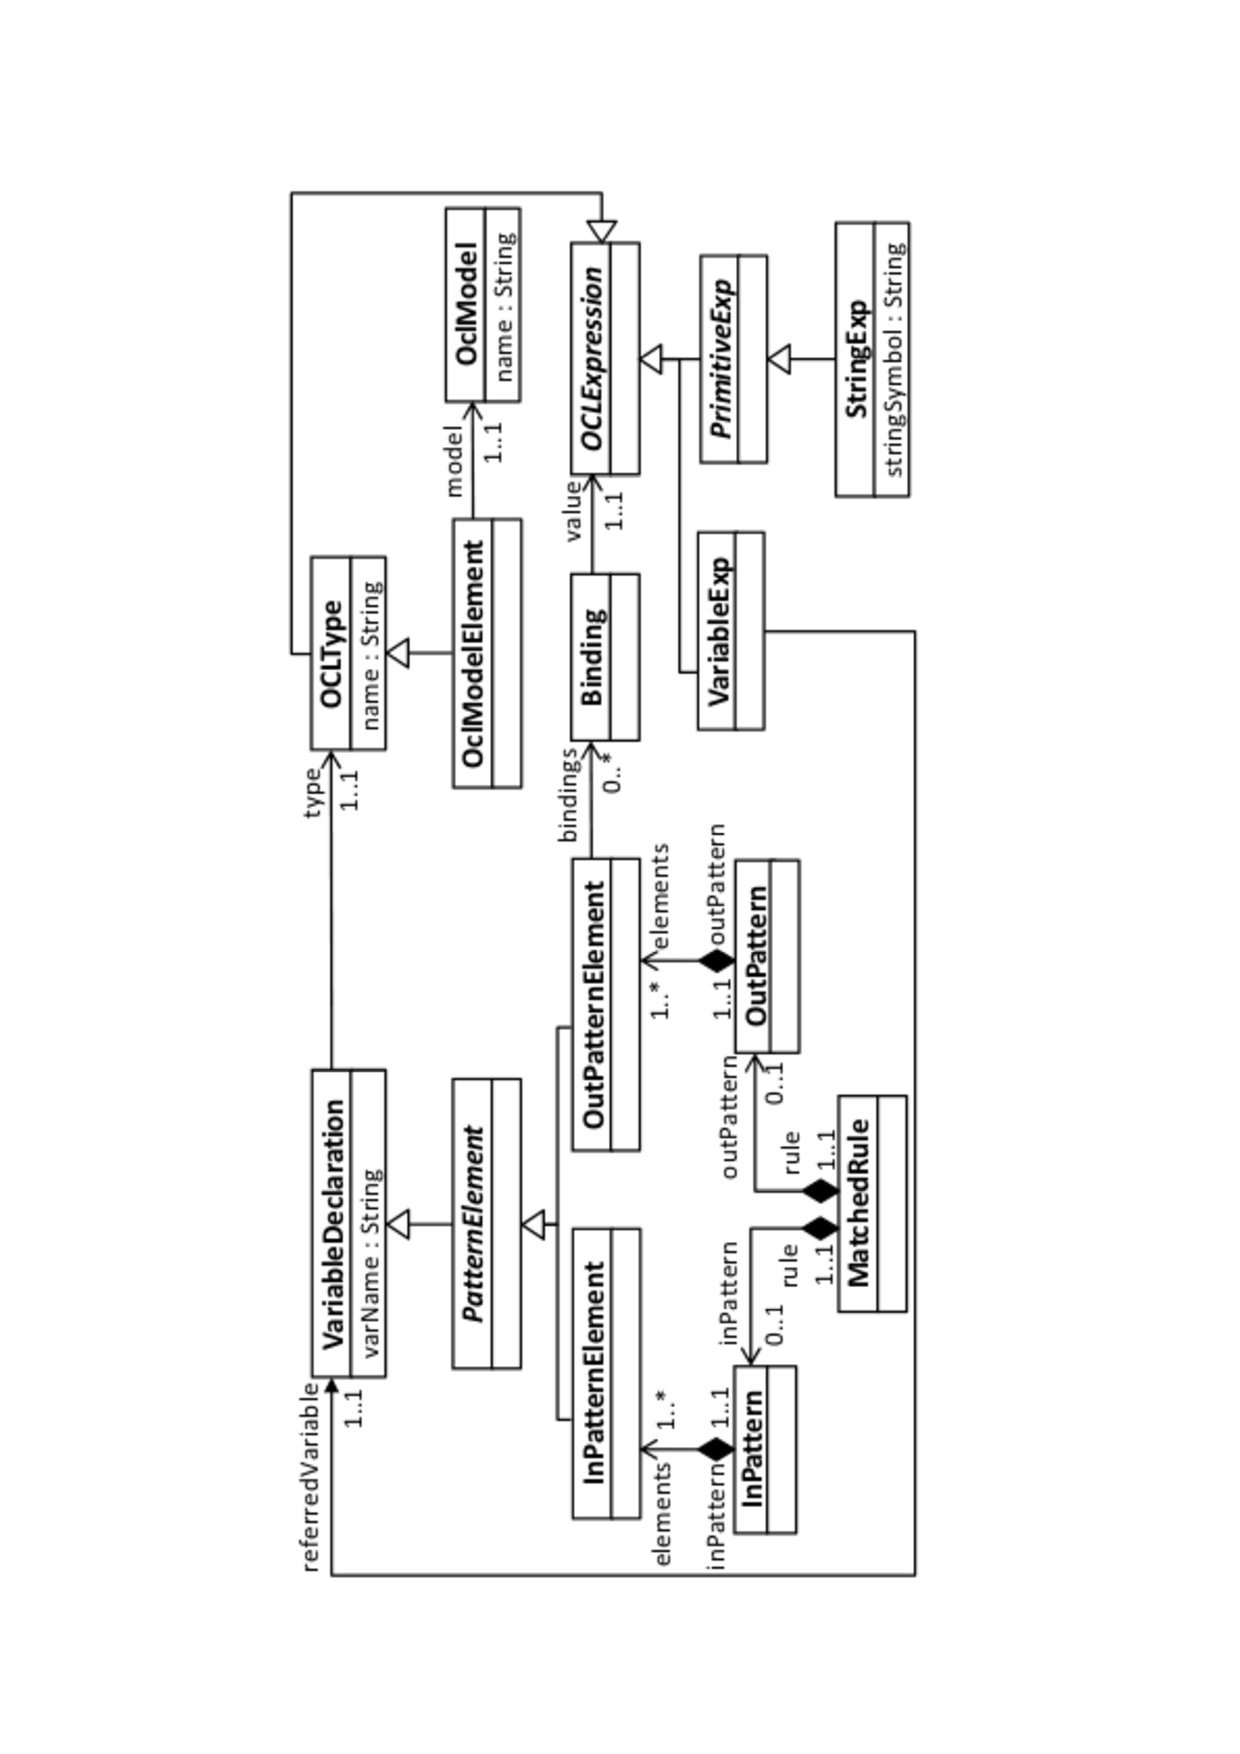
\includegraphics[angle=270,width=1\textwidth,natwidth=610,natheight=642]{figures/ATL_Metamodel_Excerpt}
	\caption{Excerpt of the ATL metamodel}
	\label{fig:atl_metamodel_excerpt}
\end{figure}

Bindings are used for the initialization of either \emph{attributes} or \emph{references}. Attributes are primitive values whereas references are relations to other models (variable expressions). Mutation \emph{1} and \emph{2} in table 2 are attribute binding mutations. \emph{3} is a reference binding mutation.

\subsubsection{Deletion}

Deleting a binding is the implicitly omitting of an attribute or reference assignment in the \emph{to}-part of the ATL rule. The example in listing~\ref{lst:delete} demonstrates the simple structure of delete bindings.

\begin{lstlisting}[language=ATL, numbers=left,xleftmargin=5.0ex, caption=Definition of Delete-Binding., label=lst:delete]
rule DeleteBinding{
  from b: ATL!Binding
  to
}
\end{lstlisting}

\subsubsection{Addition}

The addition of a binding is the introduction of a new assignment in the \emph{OutPatternElement}. This does not work for an arbitrary type as there are type constraints of the metamodel of the OutPatternElement.

Therefore the rule has to implement a type lookup to take the set of possible properties of a specific type into account. This is not possible in the HOT because the type information of the specific metamodels are missing. 

Troya et al proposed in their paper~\cite{Bergmayr:2014} second order HOTs which are applied to the result of the first HOTs. The result of the first HOTs transformations contains type information which is available in the second order HOTs.

This results is a two pass transformation:

\begin{enumerate}
	\item Add a binding with a dummy name. (e.g. NewBindingPropertyName)
	\item Lookup available bindings and replace the dummy name with an actual available one.
\end{enumerate}

Additionally the rule has to take care to prevent the same OutPatternElement to be transformed more than once by filtering out entities which already contain the dummy binding.

This proposed algorithm is showed by listing~\ref{lst:addbinding}

\begin{lstlisting}[language=ATL, numbers=left,xleftmargin=5.0ex, caption=AddBinding-Definition, label=lst:addbinding]
rule AddBinding{
  from 
  ope : ATL!OutPatternElement ( 
    ope.bindings -> forAll( b | b.propertyName <> 'NewBindingPropertyName')
  )
  to
  ope2 : ATL!OutPatternElement (
    bindings <- ope.bindings -> append(bindingNewElement)
  ), 
  bindingNewElement : ATL!Binding (
    outPatternElement <- ope2,
    propertyName <- 'NewBindingPropertyName',
    value <- newValue	
  ),
  newValue : ATL!StringExp (
    stringSymbol <- 'testvalue'
  )	
}
\end{lstlisting}

The second order HOT does a lookup for a general supertype in the metamodel. In listing~\ref{lst:addbindingnames} the rule chooses an attribute, called \emph{EStructuralFeature}, which is added to all subtypes.

\begin{lstlisting}[language=ATL, numbers=left,xleftmargin=5.0ex, caption=AddBindingNames-Definition., label=lst:addbindingnames]
rule AddBindingNames {
from b : ATL!StringExp (
    b.stringSymbol = 'NewBindingPropertyName'
)
using{
  classes : Sequence(OUT_MM!EClass) 
	= OUT_MM!EClass.allInstancesFrom('OUT_MM') 
	-> select(c | c.getESuperTypes() -> size() <= 0);
}
to b2 : ATL!StringExp ( 
  stringSymbol <- classes 
	-> first().getEStructuralFeatures() -> last().name
)	
}
\end{lstlisting}

\subsubsection{Value change}

The simpliest value change mutation is changing a primitive expression like a StringExp. The example in listing~\ref{lst:valuechangebinding1} demonstrates how to change a primitive string expression to a constant ("Hello").

This is achieved by looking up all bindings with the \emph{ATL!StringExp} type. The next step is to set it to the constant.

\begin{lstlisting}[language=ATL, numbers=left,xleftmargin=5.0ex, caption=ValueChangeBinding-Definition., label=lst:valuechangebinding1]
rule ValueChangeBinding_All{
	from
	 b : ATL!Binding (b.value.oclIsTypeOf(ATL!StringExp))
	to
	 c : ATL!Binding (
	 	value <- newStringExp
	 ),
	 newStringExp : ATL!StringExp(
	 	stringSymbol <- 'hello'	
	 )
}
\end{lstlisting}

A simple extension of the constant value change algorithm is to change the constant to a value of the actual model. The example in listing~\ref{lst:vcbconstant} changes all string expressions to the first string value of the input model. In case there's no string expression the element is ignored.

\begin{lstlisting}[language=ATL, numbers=left,xleftmargin=5.0ex, caption=ValueChangeBinding-Definition using same constant string value., label=lst:vcbconstant]
rule ValueChangeBinding_AllSameStringValue{
	from
	 b : ATL!Binding(
	 	b.value.oclIsTypeOf(ATL!StringExp) and 
		ATL!StringExp.allInstances() -> size() > 1
	 )
	to
	 c : ATL!Binding(
	 	value <- stringexpression
	 ), 
	 stringexpression : ATL!StringExp(
	 	stringSymbol <- (ATL!StringExp.allInstances() 
			-> first()).stringSymbol
	)
\end{lstlisting}

The third approach in this category was to switch the first with the last value binding. For this we fist filter only the OutPatternElements which have more than one binding and have only StringExpression bindings.

As a second step we exclude the first and the last binding from the binding-list to replace them with our new bindings with the prepend and append commands. As a third step we have to create our new binding-elements.

Such a binding element needs three values: the corresponding OutPatternElement, the property name and the value.

As outPatternElement and propertyName we take the original outPatternElement and propertyName, as value, we take the value from the last binding for our new first element and the value from the first binding for our new last element.

Important to achieve correct values is, that we use the original binding list from the "from"-clause of the rule.

\begin{lstlisting}[language=ATL, numbers=left,xleftmargin=5.0ex, caption=ValueChangeBinding-Definition using values from input models., label=lst:2ndOrderHOT]
rule ValueChangeBinding_Switch{
from
ope : ATL!OutPatternElement (
	ope.bindings 
		-> forAll(e | e.value.oclIsTypeOf(ATL!StringExp)) and
		ope.bindings -> size() > 1
)
to
ope2 : ATL!OutPatternElement (
	bindings <- ope.bindings -> excluding (ope.bindings -> first()) 
		-> excluding (ope.bindings -> last())
		-> prepend (bindingNewFirst)
		-> append (bindingNewLast)
), 
bindingNewLast : ATL!Binding (
	outPatternElement <- ope2, 
	propertyName <- (ope.bindings -> last()).propertyName,
	value <- (ope.bindings -> first()).value
),
bindingNewFirst : ATL!Binding (
	outPatternElement <- ope2,
	propertyName <- (ope.bindings -> first()).propertyName,
	value <- (ope.bindings -> last()).value	
)
	
}
\end{lstlisting}

\subsection{Implemented InPatternElement mutations}

\subsubsection{Deletion}

The deletion of an InPatternElement requires the handling of its usage in OutPatternElement bindings.

To delete an InPatternElement (IPE) it is not enough to delete only the InPatternElement itself. You have to deal at least with one important effect. The usage of this InPatternElement in the bindings of the OutPatternElements. E.g. the rule \emph{PNMLDocument} in listing~\ref{lst:pnmldoc1} contains the IPE \emph{e}. If it is deleted the usage \emph{e} in the OutPatternElement has to be handled.


\begin{lstlisting}[language=ATL, numbers=left,xleftmargin=5.0ex,label=lst:pnmldoc1]
rule PNMLDocument {
	from
		e : PetriNet!PetriNet,
		f : PetriNet!PetriNet
	to	
		n : PNML!PNMLDocument
		(
			location <- e.location,
			xmlns <- uri,
			nets <- net			
		)
\end{lstlisting}

Listing\ref{lst:pnmldoc2} shows what would happen if the OutPatternElement isn't changed too.

\begin{lstlisting}[language=ATL, numbers=left,xleftmargin=5.0ex,label=lst:pnmldoc2]
rule PNMLDocument {
	from
		f : PetriNet!PetriNet
	to	
		n : PNML!PNMLDocument
		(
			location <- .location,
			xmlns <- uri,
			nets <- net			
		)
\end{lstlisting}

In case the IPE is deleted the corresponding binding will contain an unreferred variable. This would void the generated model. To prevent this from happening all unreferred variable bindings have to be deleted in a second step in the HOT.

A possible implementation of an IPE is shown in listing~\ref{lst:IPEDef}.

\begin{lstlisting}[language=ATL, numbers=left,xleftmargin=5.0ex,label=lst:IPEDef]
rule DelteIPE {
  from ipe : ATL!InPatternElement (
    ipe.inPattern.elements -> size() > 1 and
    ipe = ipe.inPattern.elements -> last()
  )
\end{lstlisting}

Listing~\ref{lst:IPENavDef} shows another binding deletion.

\begin{lstlisting}[language=ATL, numbers=left,xleftmargin=5.0ex,label=lst:IPENavDef]
rule DelteNavigationBinding{
from b : ATL!Binding(
	b.value.oclIsTypeOf(ATL!NavigationOrAttributeCallExp) and 
	b.value.source.referredVariable.oclIsUndefined()
)
to
}
rule DeleteCollectionBinding{
from b:ATL!Binding(		
	b.value.oclIsTypeOf(ATL!CollectionOperationCallExp) and 
	b.value.source.oclIsTypeOf(ATL!NavigationOrAttributeCallExp) and 
	b.value.source.source.referredVariable.oclIsUndefined()
)
to
}
\end{lstlisting}

To delete really all of the occurences of the IPE it is necessary to delete not only the simple binding itself, also more complex occurrences like in navigation expression (ATL!NavigationOrAttributeCallExp) or collection Expressions (ATL!CollectionOperationCallExp).
As these complex expressions can be encapsulated it is neccessary to do this deletion in some kind of recursion to cover really all occurrences.

\section{Related work}
In the related work \cite{troya:2015} the authors has identified the mutations
for ATL transformation language as in chapter \textit{Mutations in Model Transformations} descripted. We have implemented a set of possible mutations in ATL they have identified. For the general part of the paper we read some other papers with different approaches.
In another referenced work \cite{book:KhanHassine} the authors has researched
how it is possible to support mutation testing in the atlas transformation
language. The authors has defined a set of mutation operators. This operators
are:

\begin{itemize}
	\item Matched to Lazy (M2L)
	\item Lazy to Matched (L2M)
	\item Delete Attribute Mapping (DAM)
	\item Add Attribute Mapping (AAM)
	\item Delete Filtering Expression (DFE)
	\item Add Filtering Expression (AFE)
	\item Change Source Type (CST)
	\item Change Target Type (CTT)
	\item Delete Return Statement (DRS)
	\item Delete Use Statement (DUS)
	\item Change Execution Mode (CEM)
\end{itemize}

The autohors approach has been validated and the results have shown that their
defined operators successfully detected insufficiency in the test suite.

\section{Conclusion and future work}
The broader goal of this work is to create an introduction to a specific field
of model driven engineering (MDE). Integral part of MDE is model transformation.\cite{Sendall:2003}. In this paper we have implemented some solutions regarding mutations in ATL. The implementation of a set of mutation operators is discussed and evaluated regarding effectiveness. We have selected some mutations in ATL like Binding (Addtion, Deletion and Change), In Pattern Element (Addition, Class change) and Out Pattern Element (Deletion, Class change). In the paper we have explain the effect of the mutations of transformtions and we see that there are many consequences. The approach presented in this paper aims at mutation of model transformations for building trust into model transformation programs using this technique. Further work will consist in deveolpment of tools for autmated mutations of model transformations. First only for ATL and second for other model transformation languages for example like QVT.

\bibliographystyle{acm}
\bibliography{references}

\end{document}
